\subsubsection{Simulation of the $x_I$ and $y_I$ Controllers}
The final design for the $x_I$ and $y_I$ translational controllers is simulated in the following. The simulations are both of the translational velocity controller and the positioning controller. A step response and the corresponding control action of each controller is shown.
%
\begin{minipage}{\linewidth}
    \begin{minipage}{0.5\linewidth}
        \begin{figure}[H]
            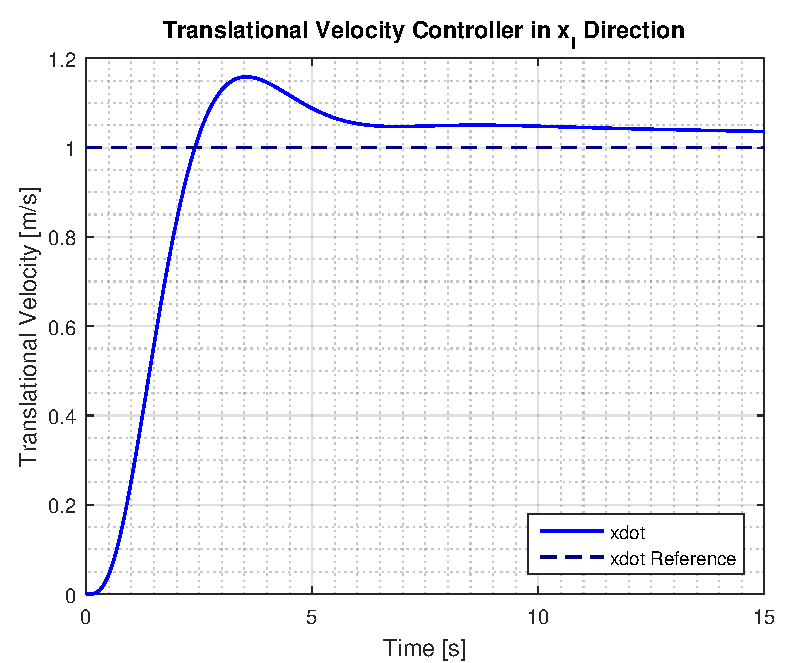
\includegraphics[scale=.58]{figures/velocityControllersXY}
            \centering			
            \captionof{figure}{A step response of the translational velocity controller in $x_I$ and $y_I$. The reference for the roll is set to one at $0.5$ \si{s} and the reference for pitch is set to one at $2.5$ \si{s}.}
            \label{fig:velocityControllersXY}
        \end{figure}
    \end{minipage}
    \hspace{0.03\linewidth}
    \begin{minipage}{0.5\linewidth}
        \begin{figure}[H]
            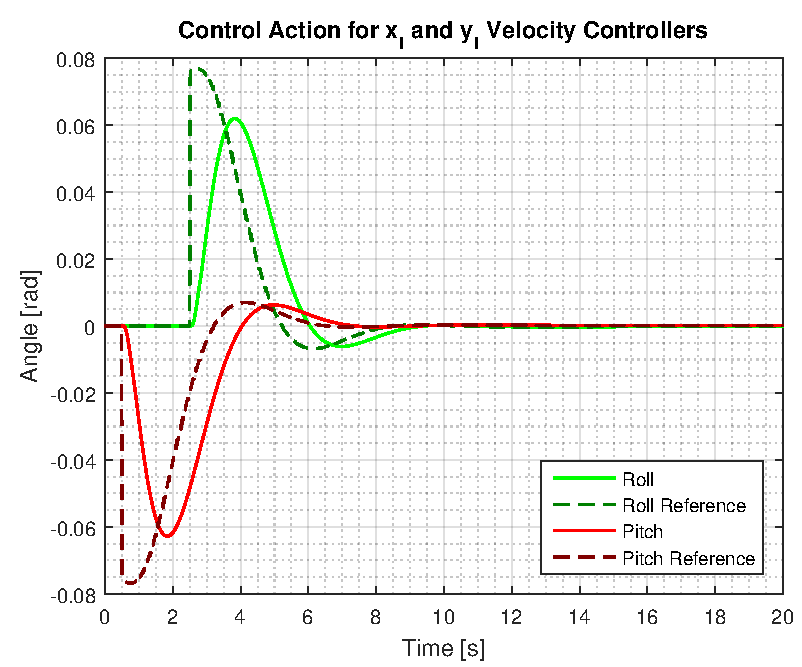
\includegraphics[scale=.58]{figures/velocityControllersXYAction}
            \centering
            \captionof{figure}{The actual control action for the actual performed step together with the required control action needed to achieve the set reference shown in \autoref{fig:velocityControllersXY}.}
            \label{fig:velocityControllersXYAction}
        \end{figure}
    \end{minipage}
\end{minipage}
%



%
\begin{minipage}{\linewidth}
    \begin{minipage}{0.46\linewidth}
        \begin{figure}[H]
            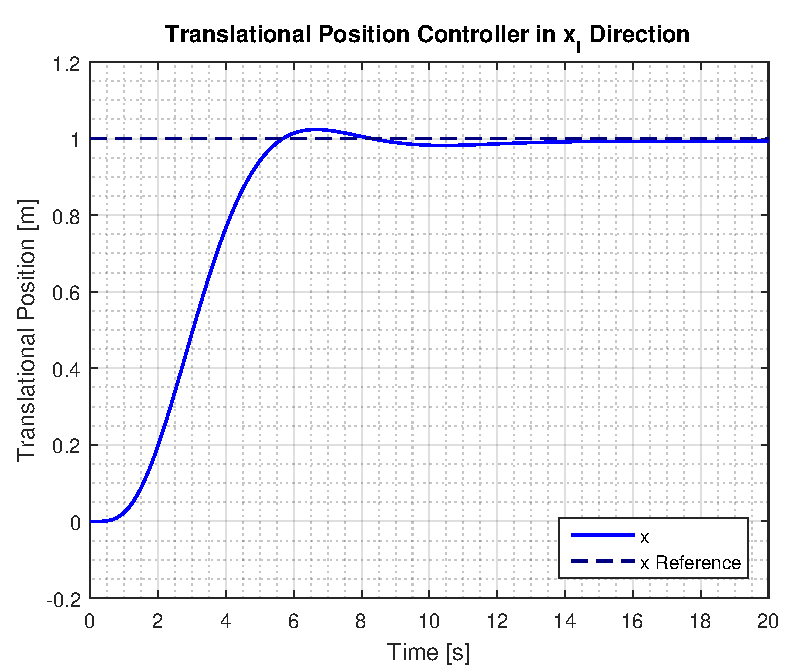
\includegraphics[scale=.61]{figures/positionControllersXY}
            \centering			
            \captionof{figure}{.}
            \label{fig:positionControllersXY}
        \end{figure}
    \end{minipage}
    \hspace{0.03\linewidth}
    \begin{minipage}{0.46\linewidth}
        \begin{figure}[H]
            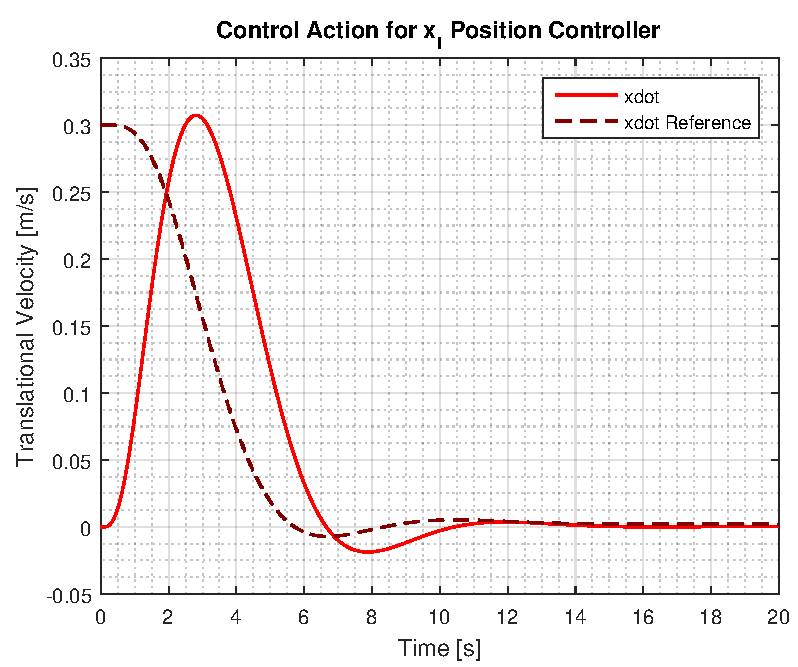
\includegraphics[scale=.61]{figures/positionControllersXYAction}
            \centering
            \captionof{figure}{.}
            \label{fig:positionControllersXYAction}
        \end{figure}
    \end{minipage}
\end{minipage}